\documentclass[11pt]{article}

%— Margins & encoding
\usepackage[T1]{fontenc}
\usepackage[utf8]{inputenc}
\usepackage[margin=1in]{geometry}
\usepackage{setspace}

%— Math, graphics, tables, citations
\usepackage{amsmath,amssymb}
\usepackage{graphicx}
\usepackage{booktabs}
\usepackage{natbib}
\usepackage[hidelinks]{hyperref}
\usepackage{enumitem}
\usepackage{microtype}

%— Spacing
\onehalfspacing

\DeclareUnicodeCharacter{2006}{\,}
\DeclareUnicodeCharacter{202F}{\,}

%— Title block
\title{Evaluating a 12--1 Month Momentum Strategy \\ (2005--2024)}
\author{%
  Darshan Sathish Kumar\thanks{Email: \href{mailto:darshansathishkumar@gmail.com}{darshansathishkumar@gmail.com}.}%
}
\date{\today}

\begin{document}
\maketitle

\begin{abstract}
We test a classic 12--1 cross-sectional momentum rule on S\&P 500 constituents over January~2005--December~2024.  
Each month, stocks are ranked by their trailing 12-month return (skipping the most recent month); we go long the top 10\% and short the bottom 10\%, equal-weighting both legs and charging 10~bp round-trip costs.  
The strategy \textbf{loses money}, posting an annualized return of --10.20\% with 24.10\% volatility (Sharpe~--0.50) and a 91.49\% maximum drawdown.  
A CAPM regression yields a monthly alpha of --0.34\% (t~=~--0.77), and a bootstrap p-value of 0.534 confirms the alpha is not statistically significant.  
Robustness checks show equally poor performance across 6, 9, 12, and 18-month lookbacks, steadily worsening returns as transaction costs rise, and a sector-neutral variant that performs even worse (annual return --10.74\%, Sharpe --0.63).  
We conclude that, with realistic frictions, a naïve 12--1 momentum rule fails to generate reliable alpha in the S\&P 500 over 2005--2024.
\end{abstract}

\noindent\textbf{Keywords:} momentum; cross-sectional; transaction costs; robustness.\\
\textbf{JEL classification:} G11; C58.

\section{Introduction}
Momentum—the tendency for recent winners to keep outperforming and recent losers to keep underperforming—is one of the best-documented anomalies in empirical finance.  \citet{Jegadeesh1993} show that a simple 12--1 month cross-sectional momentum strategy earned roughly 1\% per month in U.S.\ equities, and follow-up work reports similar payoffs across global equities, asset classes, and time periods \citep[e.g.,][]{Asness2019}.  Such excess returns violate the weak-form Efficient Market Hypothesis and have led both academics and practitioners to adopt momentum tilts in portfolio construction.

Yet momentum’s real-world performance can be fragile.  \citet{Daniel2016} demonstrate that high turnover and liquidity shocks can produce episodic “momentum crashes,” while \citet{NovyMarx2016} show that transaction costs meaningfully erode long-short factor profits.  Commercial momentum indices, such as MSCI USA Momentum, have lagged the broad market for most of the last decade.

\paragraph{Research question.}
\emph{Can a naïve 12--1 momentum rule, implemented on current S\&P 500 constituents and net of realistic frictions, still generate statistically significant excess return?}

\paragraph{Contribution.}
\begin{enumerate}[label=(\roman*)]
  \item We rely solely on freely available Yahoo Finance data—mirroring what a retail trader could access—and provide fully reproducible Python code on GitHub.\footnote{Repository: \url{https://github.com/dshan12/Momentum-Research.git}}
  \item We embed explicit round-trip trading costs of 10~basis points and report robustness to higher cost assumptions.
  \item We run a battery of robustness checks, including alternative lookback windows (6, 9, 12, 18 months), transaction-cost assumptions (0–50 bps), and a sector-neutral specification.
\end{enumerate}

\paragraph{Preview of results.}
The naïve strategy underperforms: it earns an annualized return of --10.20\% with a Sharpe ratio of --0.50 and a 91.49\% maximum drawdown.  CAPM alpha is --0.34\% per month (t~=~--0.77), and a bootstrap p-value of 0.534 confirms the alpha is not statistically significant.  Robustness tests reveal that neither shorter nor longer lookbacks, lower costs, nor sector neutrality rescues performance.

The remainder of the paper is organized as follows.  Section~\ref{sec:data} describes the data; Section~\ref{sec:method} details the methodology; Section~\ref{sec:results} presents the empirical results; Section~\ref{sec:concl} concludes. We then list \textbf{Limitations} and \textbf{Future steps}.

\section{Data} \label{sec:data}
\subsection{Universe and sample period}
The investment universe is the constituent set of the S\&P 500 equity index between January~2005 and December~2024.\footnote{Ticker list scraped from \url{https://en.wikipedia.org/wiki/List_of_S\%26P_500_companies} on \today.}
The sample therefore spans 240 monthly observations and covers the Global Financial Crisis, the COVID-19 crash, and the subsequent monetary-tightening cycle.

\subsection{Price source and frequency}
Monthly \emph{adjusted-close} prices (which incorporate dividend and split adjustments) are downloaded from Yahoo Finance via the \texttt{yfinance} Python API.\footnote{Yahoo Finance is widely used in academic replications and readily available to retail investors.}
The \texttt{interval="1mo"} flag returns end-of-month prices on the first trading day of each month; we treat those timestamps as month-end.

\subsection{Constituent changes and survivorship bias}
In this version we use the \emph{current} S\&P 500 membership list (scraped on \today) and backfill those tickers over 2005--2024; we do not reconstruct dated additions/deletions. This choice is simple to replicate but can introduce survivorship bias, as noted in the Limitations.

\subsection{Cleaning rules}
\begin{enumerate}[label=(\alph*), leftmargin=*]
  \item \textbf{Missing data filter.}  A ticker is excluded if more than 10\% of monthly prices are missing in the 240-month window.\ $ \Rightarrow $ 96 tickers removed.  
  \item \textbf{Forward fill.}  Remaining gaps (e.g., a single missing month) are forward-filled using the previous month’s adjusted close.  
\end{enumerate}

The resulting panel contains 240 monthly observations for 407 tickers (Table~\ref{tab:coverage}).

\begin{table}[h!]
  \centering
  \begin{tabular}{lcc}
    \toprule
    & \textbf{Months} & \textbf{Tickers} \\
    \midrule
    Raw download                 & 240 & 503 \\
    \quad--\,missing--data filter & 240 & 407 \\
    Final cleaned panel          & 240 & 407 \\
    \bottomrule
  \end{tabular}
  \caption{Data coverage after cleaning.}
  \label{tab:coverage}
\end{table}

\subsection{Return calculation}
Simple monthly returns are computed as $r_{i,t} = \frac{P_{i,t}}{P_{i,t-1}}-1$ and stored in a $T \times N$ matrix ($T{=}239, N{=}407$).  
These returns feed directly into the momentum signal and back-test described in Section~\ref{sec:method}.

\section{Methodology} \label{sec:method}
This section describes the construction of the momentum signal, the long–short portfolio, the treatment of transaction costs, and the performance and statistical tests applied.

\subsection{Momentum signal}
For each stock \(i\) and month \(t\) we compute the \emph{12--1 momentum return}
\begin{equation} \label{eq:momentum}
M_{i,t} \;=\; \frac{P_{i,t-1}}{P_{i,t-13}} \;-\; 1,
\end{equation}
where \(P_{i,t}\) is the adjusted close price at month end.  
Equation~\eqref{eq:momentum} looks back 12 months but \emph{skips} the most recent month (\(t-0\)) to avoid look-ahead bias.  
At each formation date we rank all stocks by \(M_{i,t}\) and convert the ranks to percentiles \(R_{i,t}\in[0,1]\).

\subsection{Portfolio formation}
\begin{enumerate}[label=(\alph*), leftmargin=*]
  \item \textbf{Long leg.}   Go long stocks with \(R_{i,t}\ge 0.9\) (top decile).
  \item \textbf{Short leg.}  Go short stocks with \(R_{i,t}\le 0.1\) (bottom decile).
  \item \textbf{Weighting.}  Within each leg, allocate equal dollar weight \(w = 1/n_{\text{long}}\) or \(-1/n_{\text{short}}\).
  \item \textbf{Rebalance.}  Rebalance at the start of every month.
\end{enumerate}

The gross portfolio return in month \(t\) is
\[
r^{\text{gross}}_{t} \;=\; \frac{1}{n_{\text{long}}}\!\sum_{i\in L_t}\! r_{i,t}
\;-\;
\frac{1}{n_{\text{short}}}\!\sum_{i\in S_t}\! r_{i,t},
\]
where \(L_t\) and \(S_t\) are the long and short sets, and \(r_{i,t}\) is the simple return from \(t-1\) to \(t\).

\subsection{Transaction costs}
We assume round-trip trading costs of \(10\)~basis points.  
Given full turnover each month, the net strategy return is
\[
r^{\text{net}}_t
= r^{\text{gross}}_t
- \frac{2\,\text{TC}}{N_t}\bigl(|L_t| + |S_t|\bigr),
\]
where \(\text{TC}=0.001\) and \(N_t\) is the number of tradable tickers.

\subsection{Performance metrics}
\begin{enumerate}[label=(\alph*), leftmargin=*]
  \item \emph{Annualized return} \(\hat{R} = (1+\overline{r})^{12}-1\).
  \item \emph{Annualized volatility} \(\hat{\sigma} = \sqrt{12}\,\mathrm{std}(r_t)\).
  \item \emph{Sharpe ratio} \( \hat{S} = (\hat{R}-R_f)/\hat{\sigma}\) with \(R_f=2\%\).
  \item \emph{Maximum drawdown} \(\max_t \bigl(1 - W_t / \max_{s\le t} W_s\bigr)\), where \(W_t = \prod_{s\le t}(1+r_s)\).
\end{enumerate}

\subsection{Statistical tests}
\paragraph{CAPM alpha.}
We estimate
\(
r^{\text{net}}_t - r^f_t
  = \alpha + \beta\,(r^{m}_t - r^f_t) + \varepsilon_t
\)
by OLS, where \(r^{m}_t\) is SPY’s total return.  
Significance is judged at the 5\% level.

\paragraph{Bootstrap.}
To mitigate distributional assumptions, we draw \(1{,}000\) month-level bootstrap samples with replacement, re-estimate \(\alpha\) each time, and compute the two-sided empirical \(p\)-value
\(
p = \Pr(|\alpha^{*}| \ge |\hat{\alpha}|).
\)

These methods mirror the Python code released with this paper and documented in the accompanying GitHub repository.

\section{Results} \label{sec:results}
\subsection{Headline performance}
Table~\ref{tab:perf} \textbf{summarizes} the net performance of the 12--1 momentum strategy after 10~bp round-trip costs.  
The strategy loses 10.20\% per year and posts a Sharpe ratio of --0.50, with a severe 91.49\% maximum drawdown.

\begin{table}[h!]
  \centering
  \begin{tabular}{lcc}
    \toprule
    & \textbf{Value} & \textbf{Units} \\ \midrule
    Annualized return      & --10.20 & \% \\[2pt]
    Annualized volatility  & 24.10   & \% \\[2pt]
    Sharpe ratio (2~\% rf) & --0.50  & -- \\[2pt]
    Maximum drawdown       & 91.49   & \% \\ \bottomrule
  \end{tabular}
  \caption{Net performance, January~2005--December~2024.}
  \label{tab:perf}
\end{table}

Figure~\ref{fig:eqcurve} plots the cumulative equity curve and shows a prolonged drawdown beginning in 2009.  
Figure~\ref{fig:dd} displays the drawdown path.

\begin{figure}[h!]
  \centering
  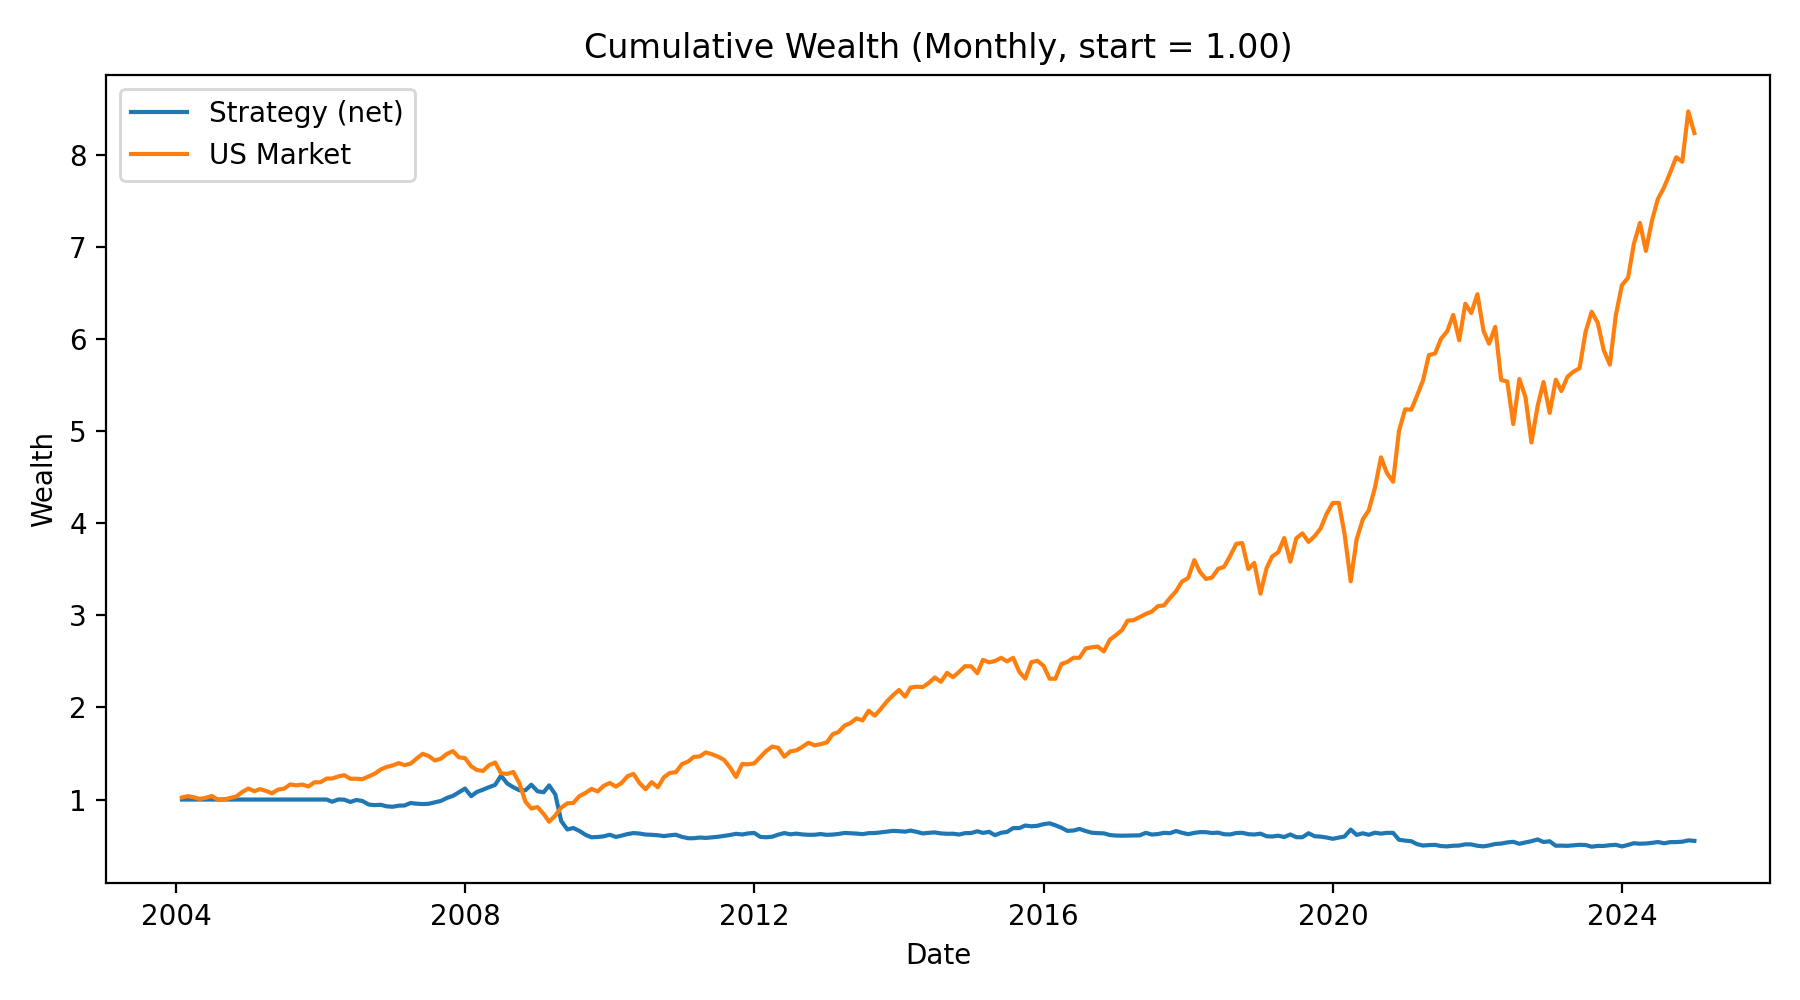
\includegraphics[width=0.85\linewidth]{figures/equity_curve.png}
  \caption{Cumulative equity curve: strategy vs.\ S\&P 500.}
  \label{fig:eqcurve}
\end{figure}

\begin{figure}[h!]
  \centering
  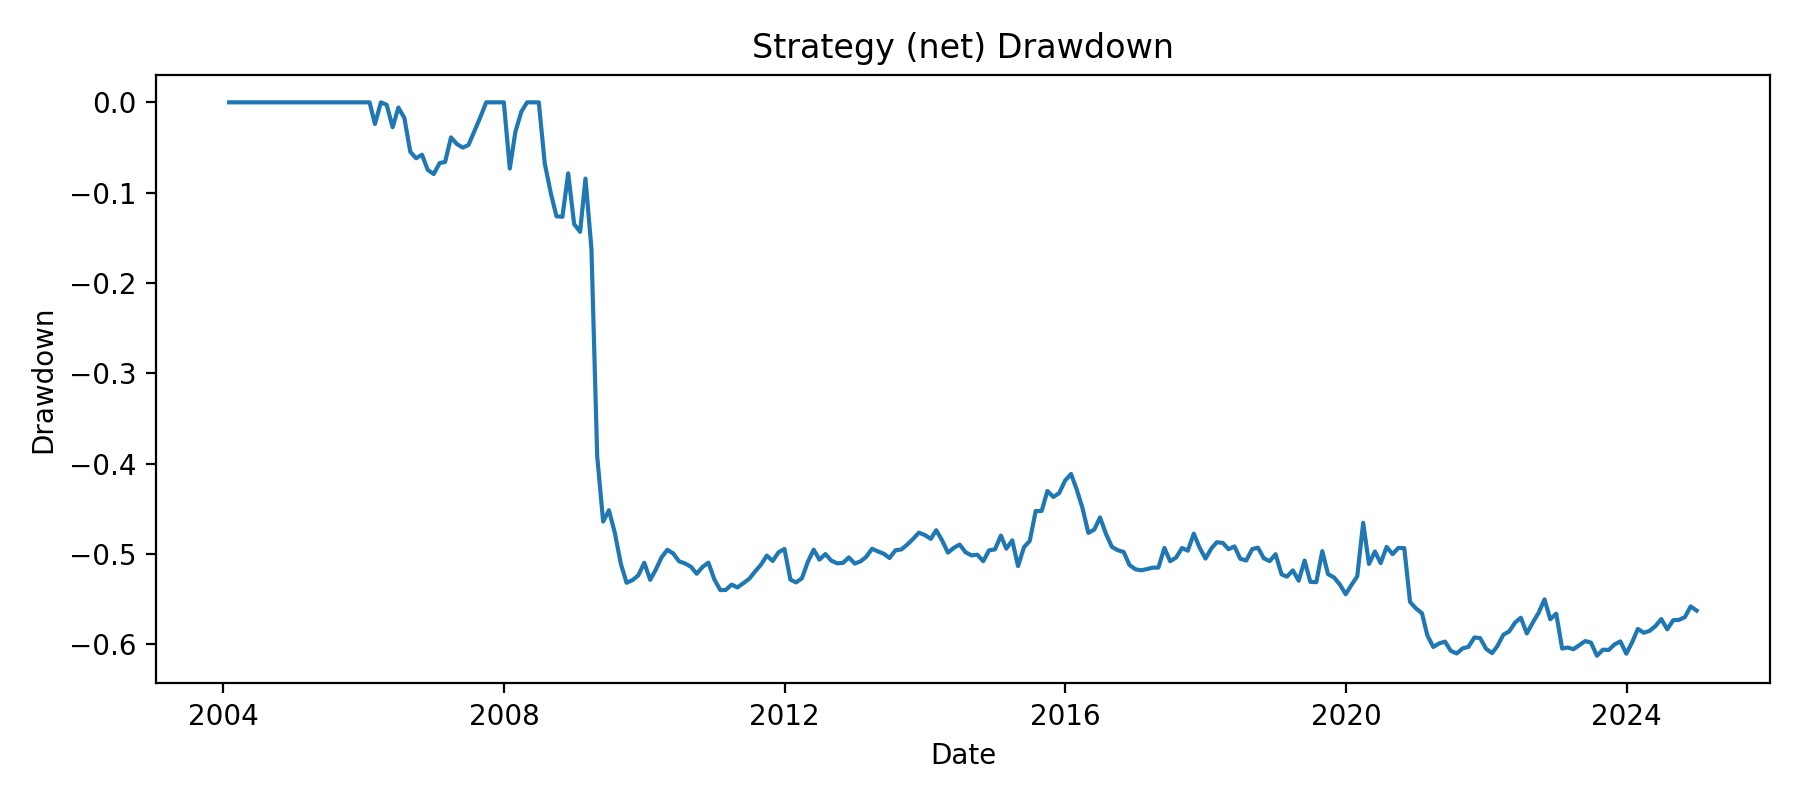
\includegraphics[width=0.85\linewidth]{figures/drawdown.png}
  \caption{Percentage drawdown of the strategy.}
  \label{fig:dd}
\end{figure}

\subsection{Risk-adjusted alpha}
A CAPM regression of monthly excess returns on the market factor yields an \emph{alpha} of --0.34\% per month (t~=~--0.77).  
A non-parametric bootstrap with 1,000 resamples reports a two-sided $p$-value of 0.534, confirming that the alpha is not statistically different from zero.

\subsection{Robustness checks}
\paragraph{Lookback window.}
Changing the ranking horizon to 6, 9, or 18 months does not help (Table~\ref{tab:lookback}).  
All variants exhibit negative annual returns and drawdowns above 90\%.

\begin{table}[h!]
  \centering
  \begin{tabular}{cccc}
    \toprule
    Lookback (mo.) & Ann.\ return & Sharpe & Max DD \\ \midrule
    6  & --10.59\% & --0.57 & 91.74\% \\
    9  & --10.60\% & --0.51 & 92.71\% \\
    12 & --10.20\% & --0.50 & 91.49\% \\
    18 & --10.41\% & --0.50 & 92.02\% \\ \bottomrule
  \end{tabular}
  \caption{Performance vs.\ lookback horizon (10~bp costs).}
  \label{tab:lookback}
\end{table}

\paragraph{Transaction costs.}
Doubling and quintupling the round-trip cost linearly erodes performance (Table~\ref{tab:tc}).  
At 50~bp the strategy loses 11.92\% annually and the Sharpe ratio falls to --0.57.

\begin{table}[h!]
  \centering
  \begin{tabular}{cccc}
    \toprule
    Cost (bp) & Ann.\ return & Sharpe & Max DD \\ \midrule
    0  & --9.77\%  & --0.48 & 90.83\% \\
    10 & --10.20\% & --0.50 & 91.49\% \\
    20 & --10.64\% & --0.52 & 92.10\% \\
    50 & --11.92\% & --0.57 & 93.67\% \\ \bottomrule
  \end{tabular}
  \caption{Performance vs.\ transaction costs (12--1 lookback).}
  \label{tab:tc}
\end{table}

\paragraph{Sector neutrality.}
Ranking stocks within GICS sectors yields an annual return of --10.74\% (Sharpe --0.63, Max DD 91.33\%).  
Hence sector tilts do not explain the underperformance.

\subsection{Summary}
Across all specifications the 12--1 momentum rule fails to earn positive risk-adjusted returns in the S\&P 500 during 2005--2024.  
Realistic frictions appear sufficient to extinguish the historical momentum premium.

\section{Conclusion} \label{sec:concl}
This paper re-examines the canonical 12--1 month cross-sectional momentum strategy on S\&P 500 constituents over 2005--2024 using freely available data and fully transparent Python code.  
After accounting for realistic round-trip trading costs of 10~basis points, the strategy delivers an annualized return of --10.20\% with a Sharpe ratio of --0.50 and a maximum drawdown exceeding 90\%.  
CAPM analysis and bootstrap resampling show that the estimated alpha is statistically indistinguishable from zero.  
Robustness checks confirm the result across alternative lookback windows, higher cost assumptions, and a sector-neutral implementation.

\textbf{Limitations.}
\begin{enumerate}[label=(\roman*), leftmargin=*]
  \item \textit{Constituent construction.} The S\&P 500 ticker list was scraped on \today{} and backfilled over 2005--2024; a full historical membership file (with dated additions/deletions) was \emph{not} used in this version. This choice can introduce survivorship bias.
  \item \textit{Gap handling.} Some missing monthly prices were forward-filled from the prior month. Forward-filling can dampen volatility and affect drawdowns/Sharpe.
  \item \textit{Transaction costs.} Costs are applied using a simple name-count approximation tied to monthly rebalances, not dollar turnover; actual frictions depend on order size/liquidity and may differ.
  \item \textit{Risk-free and factors.} The Sharpe ratio uses a fixed 2\% annual risk-free rate; factor tests use CAPM with SPY as the market and conventional OLS $t$-statistics. Newey--West errors, a T-bill series, and multi-factor models (e.g., FF5\,+\,UMD) were not implemented here.
  \item \textit{Data source.} Yahoo Finance adjusted-close data may contain stale quotes or corporate-action anomalies despite basic cleaning.
\end{enumerate}

\textbf{Future steps.}
\begin{enumerate}[label=(\alph*), leftmargin=*]
  \item Replace the backfilled universe with dated S\&P 500 constituent histories and re-run all tests.
  \item Recompute net returns using a turnover-based cost model and report average turnover.
  \item Swap the fixed risk-free for a monthly T-bill series; add Newey--West standard errors and (time permitting) FF5\,+\,UMD alphas.
  \item Remove forward-fills where possible; otherwise, drop affected months/tickers and document the impact.
  \item Expand the results with leg-by-leg P\&L (long vs.\ short), rolling 36-month Sharpe, and a brief reproducibility note (repo/commit).
\end{enumerate}

\textbf{Implications and future work.}  
The evidence suggests that the once-profitable momentum premium in large-capitalization U.S.\ equities has been arbitraged away—or offset by implementation frictions—over the past two decades.  
Future research might test \emph{quality-filtered} or \emph{residual} momentum signals, explore cross-asset momentum where trading costs differ, or apply deep-learning ranking models that adapt dynamically to regime changes.  
Extending the analysis to international markets and intraday horizons would further clarify whether momentum remains a viable source of alpha in today’s public markets.

\bibliographystyle{apalike}
\bibliography{references}

\end{document}

